\chapter{Introduction}

% \todo{Findes der klasser af problemer hvor GPen fejler? Hvad karakterisere de klasser?, Mere blødt, undersøg
% Kig på functions klasser. }

% Introduction section
%  1. Introduction.
%  2. Background and setting. 
%  3. Identification of problem
%  4. Purpose Statement. 
%  5. Objectives or research questions
%  6. Assumptions. Limitations. Definition of terms
%  7. Significance of the study.

% Introduction section (from unsw.edu.au)
% Move A: establish your territory (say what the topic is about)
%   1.  state the general topic and give some background
%   2.  provide a review of the literature related to the topic
%   3.  define the terms and scope of the topic
Optimization plays an important role in our everyday life, science development, product design, and
much more. Examples of optimization could be choosing the optimal way to commute from A to B,
deciding what songs should land on your playlist, or constructing the strongest possible bridge
using limited material. In general, optimization is the methodology of choosing the best decision
among a set of possible decisions. Often we try to quantify how good a decision is: A specific bus
takes 20 min to go from A to B, you rate a specific song 4 out of 5, and a particular bridge design
costs 10 million DKK. Suppose it is possible to come up with a quantification of how good a
decision is in terms of a real number. In that case, we can formulate the optimization problem as
a \textit{mathematical optimization problem} \cite[1]{boyd2004convex}: 
$$\min_{x\in \mathcal{X}} f(x),$$ where the functional $f: \mathcal{X} \rightarrow \mathbb{R}$ is
called the \textit{objective function} and $\mathcal{X}$ is the set of possible decisions.
Throughout this thesis, we refer to optimization as minimizing the objective function. Solving the
mathematical optimization problem is an active research field, and many algorithms have been
developed to find the minimum of the function $f(\cdot)$ \cite{boyd2004convex}.

Evaluation of the objective function can be cheap (e.g., if it just requires summing/multiplying
numbers) or highly expensive (e.g., if it involves human rating, large simulation, or physical
experiments). In the latter case, we want to avoid evaluating the objective function as much as
possible - we want to use \textit{sample-efficient} optimization. The overall topic of this thesis,
\textit{Bayesian optimization} (BO), is one of the preferred frameworks for sample-efficient
optimization \cite{TakeHumanOutOfLoop}.
%maybe mention more?

Bayesian optimization is a probabilistic surrogate-based optimization methodology: Assuming some
initial samples $\{(x_1,f(x_1)), \dots, (x_n,f(x_n))\}$ from a highly expensive objective, a cheap
(surrogate) function is fitted to the samples. The next sample is found by
minimizing the surrogate, and the process is repeated. Bayesian optimization seeks to enhance this
procedure with probability theory, where the surrogate function becomes a probabilistic (Bayesian)
regression model. The most common surrogate model is a Gaussian Process (GP), as it encapsulates the
uncertainty very well, and its inference procedure (computing answers to probability queries like
$p(y|x)$) is exact. %MÅSKE OMFORMULER?

% Move B: establish a niche (show why there needs to be further research on your topic)
%   4.  outline the current situation
%   5.  evaluate the current situation (advantages/ disadvantages) and identify the gap

Even though GP has proven suitable for many cases, there will be problems where its assumptions do
not hold. For example, the commonly seen GP with an isotropic kernel (covariance between two points
is invariant to translation in input) yields a strong assumption about the continuity of the
objective function and that the objective function behaves similarly throughout the domain
$\mathcal{X}$. In Figure \ref{GP_vs_BNN} we see an example of how the GP's uncertainty
quantification becomes unreasonable due to a discontinuity in the underlying objective function. In
some areas, it is prevalent to have these discontinuities, for instance, in material discovery
\cite{Nature_BO_paper}. To accommodate the strong assumptions of the GP the literature introduces
more flexible kernel functions; however, this introduces additional hyperparameters. Since we often
only deal with a small amount of data, tuning and computation of these more complex GPs can be
significantly challenging \cite{Nature_BO_paper}.

% make better figure!
\begin{figure}[H]%
    \centering
    \subfloat{{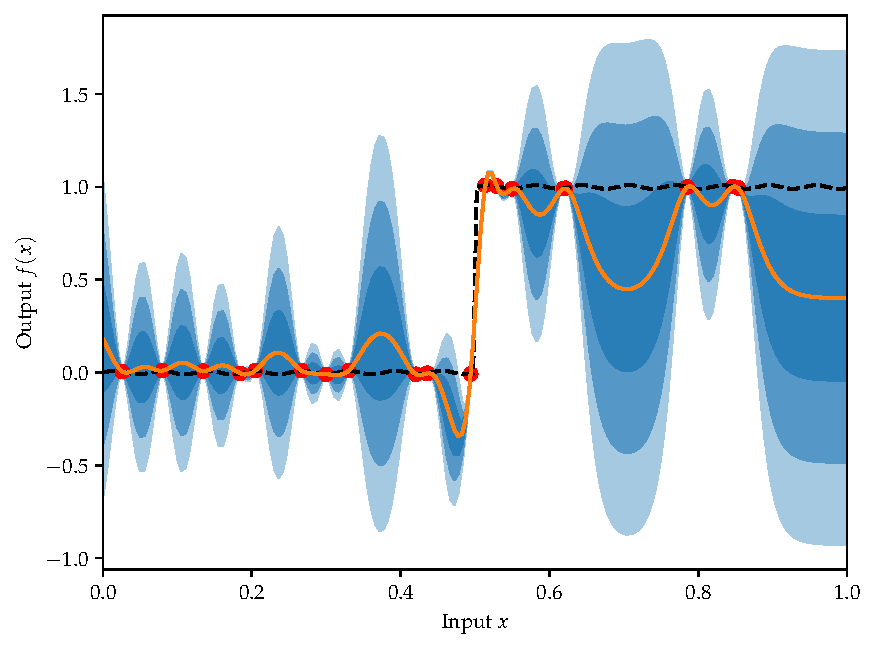
\includegraphics[trim=0.1cm 0.3cm 0.2cm 0.2cm,clip,width=0.46\textwidth]{Pictures/GP_vs_BNN1_b.pdf} }}%
    \qquad
    \subfloat{{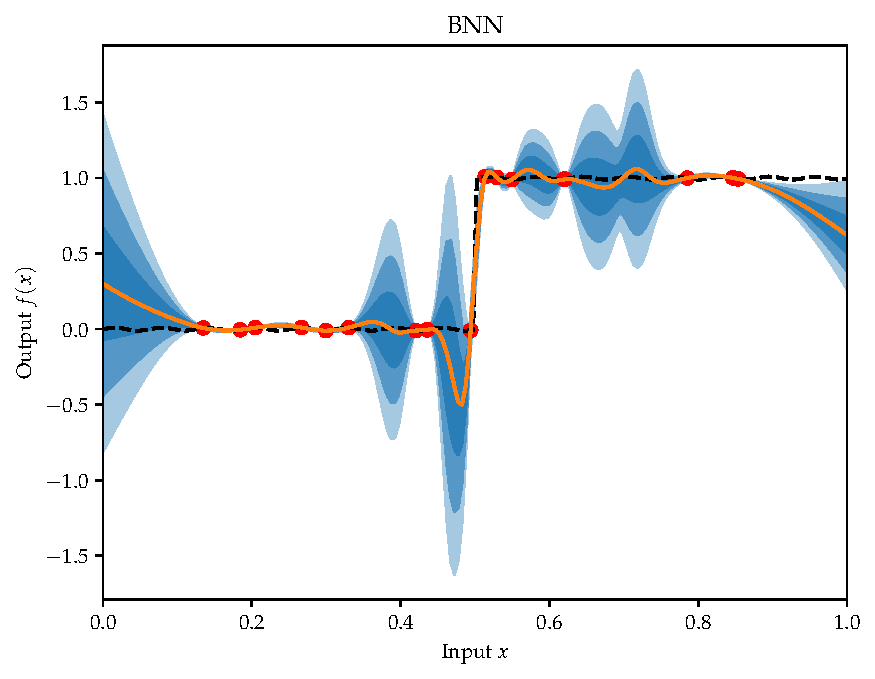
\includegraphics[trim=0.1cm 0.3cm 0.2cm 0.2cm,clip,width=0.46\textwidth]{Pictures/GP_vs_BNN2.pdf} }}%
    \caption{Gaussian process (GP) and Bayesian neural network (BNN) fitted to 18 data points. The objective function is the
    dashed black line. This examplifies how a discontinuity makes the standard implemented GP
    (optimized with emperical Bayes) expresses large uncertainties to all other areas in the domain $[0,1]$, while the
    Bayesian NN only express uncertainty where the discontinuity happens at $x =
    0.5$}\label{GP_vs_BNN}
\end{figure}


% Move C: introduce the current research (make hypotheses; state the research questions)
%   6.  identify the importance of the proposed research
%   7.  state the research problem/ questions
%   8.  state the research aims and/or research objectives
%   9.  state the hypotheses
%   10. outline the order of information in the thesis
%   11. outline the methodology

GPs are attractive models since they allow for exact inference, a closed-form expected improvement
 (see Section \ref{ExactEI}) and, in general, provide a satisfying uncertainty quantification.
 However, as we saw in the Figure \ref{GP_vs_BNN} we can maybe do better --- especially if we have
 some insights into the behavior of the objective function (i.e. yielding a more transparent
 black-box optimization problem). A better surrogate model ultimately implies fewer samples to reach
 an optimal solution, and can, thereby, potentially save work hours, money, or energy. Therefore,
 the investigation of the performance of other surrogate models is highly relevant. In this thesis,
 we aim to create surrogate models alternative to GPs, which can perform better on certain classes
 of (complex) problems, and have comparable performance on most classes of problems. 

 \section{Project limitation and contibution}
Even though it would be interesting to examine different types of GPs such as deep kernel
learning \cite{deepkernel}, we limit the scope of this project to deal with the following surrogate models:
\begin{itemize}[noitemsep]
    \item GP with Matérn kernel
    \item Bayesian neural network (BNN)
    \item Mixture regression (Gaussian mixture model, kernel density estimator, sum-product networks)
\end{itemize}
and we choose only to test the Bayesian optimization with the widely used acquisition function:
\textit{expected improvement}. Furthermore, we only deal with problems in continuous domains
$\mathcal{X} \in \mathbb{R}^m$. The proposed hypothesis is,

\begin{enumerate}[noitemsep]
    \item Mixture regression models and BNNs can be effective surrogate models
    performing better than GPs in some complex BO problems. 
\end{enumerate}

Note that we here use "performance" to describe \textit{sample efficiency}, i.e., how few evaluations/samples
of the objective function are necessary to find the minima. So here, it is assumed that the objective
function is so expensive (whatever that means to the stakeholder) that its cost outweighs the power
and time spent on the surrogate modeling and optimization.


We test the performance of the surrogates models on 4 self-made problems and 

% 1) Firstly, we want to examine what types of problems a GP surrogate is not a good choice and
% where Bayesian neural nets (BNN) surrogates can have an advantage (inspiration found in this 2020
% thesis \cite{PhDthesis})
    
% 2) Looking at sum product networks (SPN) as novel surrogate models. A SPN is - similarly to a BNN
% - a deep probabilistic model and still expressive but with tractable inference, which potentially
% could lead to advantages over BNNs. 

\section{Related work}
\todo{Might delete this}
Here we give a short overview of research in different surrogates for Bayesian optimization
and the very related field of active learning. The different surrogate models, which are in the 
research we found, 

Mostly the work done on surrogate models are 



\begin{itemize}[noitemsep]
    \item Gaussian process
    \item Bayesian neural network
    \item Random forest regression
    \item Kernel density estimator
    \item Bayesian multivariate adaptive regression splines (BMARS)
    \item Bayesian additive regression trees (BART)
\end{itemize}

Since inference time of the GP scales cubic with the number of samples, often research in
alternative surrogate models has its primary focus on lowering the computational complexity of
inference while showing the sample efficiency is (or almost is) as good as the GPs. A popular model
in the current time is a (deep) neural network and using a neural network as a probabilistic
surrogate model (i.e. Bayesian Neural Network \cite{BOHAMIANN} or as basis functions in linear
regression \cite{DNGO}) yields only linear complexity. However, as mentioned above, this thesis
assumes that the objective function is always more costly than the inference cost. And cubic
complexity for a GP does not matter for the small number of samples, which is often the case for
highly expensive Bayesian optimization problems. 

Inference complexity is also the main focus of the Ph.D. thesis "Sample-efficient Optimization Using
Neural Networks" from 2020 \cite{PhDthesis}, but his chapter 3 showcases empirically that using Bayesian
neural networks as surrogate models performed better, or at least comparable to GPs on a wide number
of problems. The performance difference was more evident for high-dimensional problems.

The 2021 paper "Bayesian optimization with adaptive surrogate models for automated experimental design"
\cite{Nature_BO_paper}, focus on the sample efficiency of the BO applied to autonomous materials discovery, 
which yields a relatively high-dimensional design space and non-smooth patterns of objective functions.  
The paper shows that using Bayesian multivariate adaptive regression splines
and Bayesian additive regression trees as alternative surrogate models outperform GP significantly, 
for complex BO problems. 

Active learning is closely related to Bayesian Optimization, but here the focus is on learning the
underlying function using as few samples as possible instead of just finding its minima. In active
learning, a Gaussian process is also very common, but the paper "Active Learning with Statistical
Models" \cite{ALStatisticalModels} investigates using Gaussian mixtures and kernel estimator in
active learning, i.e. as a surrogate model for selecting the next samples. These regression
models are not seen much in the literature; They are modeling the joint distribution of x and y, and
using the conditional distribution $p(y|x)$ as the regression model. The results were ... ??

\section{Structure of this thesis}
The structure of this thesis is as follows: Firstly, build up the foundation around Bayesian
optimization. Secondly, present different surrogate/Bayesian regression models. Thirdly, show the
results on different types of problems on Bayesian regression performance and on Bayesian
optimization performance. Finally, a discussion and conclusion are presented. In more detail the different
chapters are, 

\begin{enumerate}[noitemsep]
    \item \textbf{Introduction}
    \item \textbf{Bayesian optimization}: First we establish the relevance for BO as a
    sample-efficient solver. Secondly, we explain the two components of BO: A 
    surrogate/Bayesian regression model and an acquisition function.
    \item \textbf{Discriminative models surrogates}: Gaussian processes and Bayesian neural
    networks are presented and discussed in terms of inference procedures and regression performance. 
    \item \textbf{Generative models as surrogates}: Since the mixture models are not 
    inherently Bayesian, we present the conditional distribution in a Bayesian setting. 
    Next, the three different mixture regression models are presented: Kernel density regression, Gaussian mixture regression,
    and the novel (in a regression setting) Sum-product networks.
    \item \textbf{Results}: Testing regression and Bayesian Optimization performance
    (sample-efficiency) on 4 homemade test functions and the popular benchmark COCO.
    \item \textbf{Discussion} and \textbf{conclusion}
\end{enumerate}

% \begin{itemize}
%     \item The first chapter introduces the concept of optimization in general, Bayesian optimization 
%     and how surrogates/Bayesian regression models are relevant.
%     \item The second chapter introduces GP and Bayesian Neural Networks
%     \item The third chapter introduces the mixture regression and the novel SPN regression.
%     \item The fourth chapter results
%     \item Finally a discussion and conclusion.
% \end{itemize}


\section{Notation}
Following is the general notation used in this thesis, but some chapters (e.g. about GPs) will alter the notation a bit. 
\begin{itemize}[noitemsep]
    \item $y \in \mathbb{R}$: Observation or sample of $f(x)$ (potentially with noise).
    \item $f(\cdot): \mathcal{X} \rightarrow \mathbb{R}$: Objective function.
    \item $x \in \mathcal{X}$: Location or point in the sample space.
    \item $\textbf{x}$: Set of location or points in the sample space.
    \item $\textbf{y}$: Set of observations or samples for corresponding $\textbf{x}$.
    \item $\mathcal{D}$: Collection of samples in the optimization landscape. 
    \item $\mathcal{N}(x|\mu, \Sigma)$: The density of a normal distribution evaluated in $x$.
    %\item $\mathcal{Cat}(x|\alpha_1, \dots, \alpha_k)$: The density of a catagorical distribution evaluated in $x$.
    \item \textit{optimization landscape}: joint set of points in the domain and the objective function
    evaluated in the points, i.e. $\{(x,f(x))\in \mathcal{X} \times \mathbb{R}| x \in \mathcal{X}\}$.
    \item $y \sim p(y)$: A realization of $y$ with the density $p(y)$
\end{itemize}

\subsection{Bayesian notation}
Throughout this thesis we will be using Bayesian notation, i.e. $p(x) := P(X=x)$ is the probability
density function of the random variable $X$ evaluated in $x$ and $p(y|x) := P(Y=y|X=x)$. %or $p(y|x):= P(Y|X=x)$. 
Furthermore, writing $p(y^2|x)$ means $P(Y^2=y^2|X=x)$ and \textbf{not} $P(Y=y^2|X=x)$. 
Another noteable notation is the expecation of $g(y)$ with respect to the preditive distribution 
$$E_{p(y|x,\mathcal{D})}[g(y)] = \int g(y) p(y|x,\mathcal{D}) dy.$$
% \begin{itemize}[noitemsep]
%     \item Expecation of $g(y)$ with respect to the preditive distribution, $E_{p(y|x,\mathcal{D})}[g(y)] = \int g(y) p(y|x,\mathcal{D}) dy.$
%     \item Predictive variance,$V_{p(y|x,\mathcal{D})}[y] = E_{p(y|x,\mathcal{D})}[y^2]-E_{p(y|x,\mathcal{D})}[y]^2.$
% \end{itemize}
% \begin{align*}
%     &E_{p(y|x,\mathcal{D})}[g(y)] = \int g(y) p(y|x,\mathcal{D}) dy &:&\text{Expecation of $g(y)$ w.r.t. the preditive distribution}\\
%     &V_{p(y|x,\mathcal{D})}[y] = E_{p(y|x,\mathcal{D})}[y^2]-E_{p(y|x,\mathcal{D})}[y]^2 &:&\text{Predictive variance}
% \end{align*}

% We will refer to $y$ as an observation or sample at a given location or point $x$. This terminology will fit into the intuitive
% way of understanding an optimization problem as a (high dimensional) \textit{landscape}, 
% where the objective function is the altitude in the landscape. 
% We refer to \textit{optimization landscape} as the joint set of points in the domain and the objective function
% evaluated in the points, i.e. $\{(x,f(x))\in \mathcal{X} \times \mathbb{R}| x \in \mathcal{X}\}$. Since
% the evaluation of $f(\cdot)$ might be noisy or inprecise, we just observe $y = observe(x)$. The typical
% connection between $f(x)$ and $y$ are $y = f(x)$ or $y = f(x) + \epsilon$, where $\epsilon$ is additive white noise, 
% but different connections might be present as well. 
